\chapter{Introduction}

As computers steadily become vital tools in our day-to-day lives, the need arises to extend the ability to develop computer applications to ampler audiences, including those who lack a programming background.
OutSystems~\cite{outsystems-website} is a low-code development platform that enables its users to build applications through a graphical interface and integrate them with existing systems. It speeds up the development of web and mobile applications, at the same time making the task more accessible to users from different backgrounds.

Data analysis is a powerful resource with various applications that has flourished as a research field over the years.
%Naturally, data collection is a pivotal step in performing any kind of data analysis.
Digital forms are increasingly popular tools for structured data collection. They can gather large amounts of data from users all across the globe in a short amount of time. Furthermore, in digital forms, we can perform real-time validations on the input fields.
%\textcolor{purple}{Digital forms can be used to collect structured data while performing real-time validations on the input fields.}
Well-written validations result in overall cleaner and standardised data, free of invalid values, such as typographical mistakes (`typos') and format inconsistencies, which requires less processing to ready for analysis.

Regular expressions (also known as regexes) are powerful mechanisms for describing patterns in text with numerous applications.
One notable use of regular expressions is precisely to perform form validations on the input fields of digital forms.
%
Aside from validating the format of form input strings, regular expressions can be coupled with capturing groups.
%
A capturing group is a sub-regex within a regex that is indicated with parenthesis and 
captures the text matched by the sub-regex inside them.
Capturing groups are used to extract information from text and, in the domain of form validation, they can be used to enforce conditions over values in the input string.

One of the many features offered by OutSystems is the automatic generation of forms based on a high-level description of desired fields, to which users can subsequently add custom hand-written validations that are checked before the form is submitted.
%
Its usefulness notwithstanding, form validations often rely on complex regular expressions which require programming skills that not all users possess.
Furthermore, hand-written validations are error-prone. Programmers often miss corner cases, admitting less-than-obvious mistakes that more imaginative form-fillers may commit.

Program synthesis is the task of automatically generating a program that satisfies some desired behaviour expressed as a high-level specification.
Since low-code platforms have the ultimate vision of making application development accessible to everyone, there is a lot of potential in the integration of program synthesis in such platforms.
Owing to its versatility and usefulness, program synthesis has recently attracted interest from various research communities (e.g.
constraint solving \cite{DBLP:conf/ijcai/KolbTPR18,Orvalho19,DBLP:journals/pacmpl/Yaghmazadeh0DD17,UnchartIt20,Regel20,DBLP:conf/tacas/AhmedPA20}, 
programming languages \cite{DBLP:conf/pldi/FengMBD18,DBLP:conf/pldi/FengMGDC17,DBLP:conf/pldi/WangCB17},
machine learning \cite{DBLP:conf/icml/MenonTGLK13,DBLP:conf/ijcai/EllisG17,DBLP:conf/cav/ChenWBDF20},
and deep learning \cite{DBLP:conf/iclr/BalogGBNT17,DBLP:conf/iclr/ParisottoMS0ZK17,DanielThesis,Regel20,DBLP:conf/naacl/HuangWSYH18}), leading to various promising proposals. %Nevertheless, to the best of our knowledge, there has been no effort to synthesise form validation logic.



To help users write regular expressions, prior work has proposed to synthesise regular expressions from natural language~\cite{Regel20,DBLP:conf/naacl/KushmanB13,DBLP:conf/emnlp/LocascioNDKB16,DBLP:conf/emnlp/ZhongGYPXLLZ18,DBLP:journals/pacmpl/Yaghmazadeh0DD17} or from positive and negative examples~\cite{Regel20,DBLP:conf/popl/Gulwani11,AlphaRegex16,Fidex16}. Even though these techniques assist users in writing regular expressions for search and replace operations, they do not specifically target digital form validation and do not take advantage of the structured format of the data.

\todo{Move to motivating example?}
In this thesis, we propose \Forest{}, a new program synthesizer for regular expressions that targets digital form validations.
\Forest takes as input a set of examples and returns a regex validation that validates them.
\Forest accepts three types of examples:
\begin{enumerate}%[label=(\roman*)]
    \item \textbf{valid examples}: correct values for the input field. The valid examples can be accompanied by \textbf{captures}, substrings of the examples that capture relevant information;
    \item \textbf{invalid examples}: incorrect values for the input field due to their \textit{format}, and
    \item \textbf{conditional invalid examples} (optional): incorrect values for the input field due not to their format but to their \textit{values}.
\end{enumerate}
%
\Forest outputs a regex validation, consisting of three components:
\begin{enumerate}%[label=(\roman*)]
    \item a \textbf{regular expression} that matches all valid and none of the invalid examples and
    \item \textbf{capturing groups} that reflect the captures provided with the valid examples;
    \item \textbf{capture conditions} that express integer conditions for values in the examples that are satisfied by all valid but none of the conditional invalid~examples.
\end{enumerate}

\section{Motivating Example}\label{sec:motivating-example}

Suppose a user is writing a form where one of the fields is a date that must respect the format DD/MM/YYYY.
The user wants to accept the input strings (valid examples):
\begin{multicols}{3}
    \begin{itemize}[label={}]
    \item 19/08/1996
    \item 26/10/1998
    \item 22/09/2000
    \item 01/12/2001
    \item 29/09/2003
    \item 31/08/2015
    \end{itemize}
\end{multicols}
\noindent
But not (invalid examples):
\begin{multicols}{3}
\begin{itemize}[label={}]
\item 19/08/96
\item 26-10-1998
\item 22.09.2000
\item 1/12/2001
\item 29/9/2003
\item 2015/08/31
\end{itemize}
\end{multicols}
\noindent
A regular expression can be used to enforce this format. However, if the user is not proficient in the usage of this formalism, writing it can be a challenging task. Even if the user is familiar with regular expressions, writing a large number of such validations for all the fields of a form can become monotonous and error-prone.
Instead, the user may simply use the two sets of examples as input to \Forest{}, who outputs the regular expression \UseVerb{date2}.

Suppose the user wants to validate not only the format, but also the values in the date.
We consider as \textit{conditional invalid}:
\begin{multicols}{3}
    \begin{itemize}[label={}]
    \item 33/08/1996
    \item 26/00/1998
    \item 22/13/2000
    \item 00/12/2001
    \item 12/31/2003
    \item 52/03/2015
    \end{itemize}
\end{multicols}
To ensure only valid values are inserted as the day and month, one can use capturing groups. A capturing group is represented by a set of parenthesis. They capture the text matched by the regex inside them, that can later be used with a numbered reference. In this document we use the notation \(\$i, i \in 0, 1, ...\) to reference the integer value captured by the \((i+1)\)\textsuperscript{th} group.
Then, conditions can be applied to these values. In this situation, the desired validation (and the output of \Forest) includes the same regular expression as before, now extended with two capturing groups and four integer conditions over them:
\UseVerb{date_day_mo_caps}, \(\$0 \le 31 \wedge \$0 \ge 1 \wedge \$1 \le 12 \wedge \$1 \ge 1\).

Finally, suppose the user wishes not only to validate the input string but also to extract some information from it. Still using the dates example, the user could wish to extract the year from each date, so it could be used afterwards.
\begin{multicols}{3}
    \begin{itemize}[label={}]
    \item 19/08/1996, 1996
    \item 26/10/1998, 1998
    \item 22/09/2000, 2000
    \item 01/12/2001, 2001
    \item 29/09/2003, 2003
    \item 31/08/2015, 2015
    \end{itemize}
\end{multicols}

Using a capture group, we can extract the year from each date. If the user provides these example captures alongside the valid examples, \Forest also outputs the regular expression and captures \UseVerb{date_year_cap}. The captured text corresponds to the desired information.

\section{Contributions}

As we can see in the motivating example, data inserted into digital forms is usually structured and shares a common pattern among the valid examples.
In this example, the data has the shape \texttt{dd/dd/dddd} where \texttt{d} corresponds to a digit. 
%This contrasts with general regexes for search and replace operations that are often performed over unstructured text. 
\Forest takes advantage of this structure by automatically detecting these patterns and using a divide-and-conquer approach to split the expression into simpler sub-expressions, solving them independently, and then merging their information to obtain the final regular~expression.
Additionally, \Forest computes a set of capturing groups over the regular expression, which it then uses to synthesise integer conditions that further constrain the accepted values for that form field.

% Unlike regular expressions,
Input-output examples do not require specialised knowledge and are accessible to users.
However, there is one downside to using examples as a specification: they are ambiguous. There can be solutions that, despite matching the examples, do not produce the desired behaviour in situations not covered in them.
The ambiguity of input-output examples raises the necessity of selecting one among multiple candidate solutions.
%
%To increase the confidence that the regex returned by \Forest matches the user intent,
To this end, we incorporate a user interaction model based on distinguishing inputs
for both the synthesis of the regular expressions and the synthesis of the capture~conditions. 

\begin{figure}
    \centering
    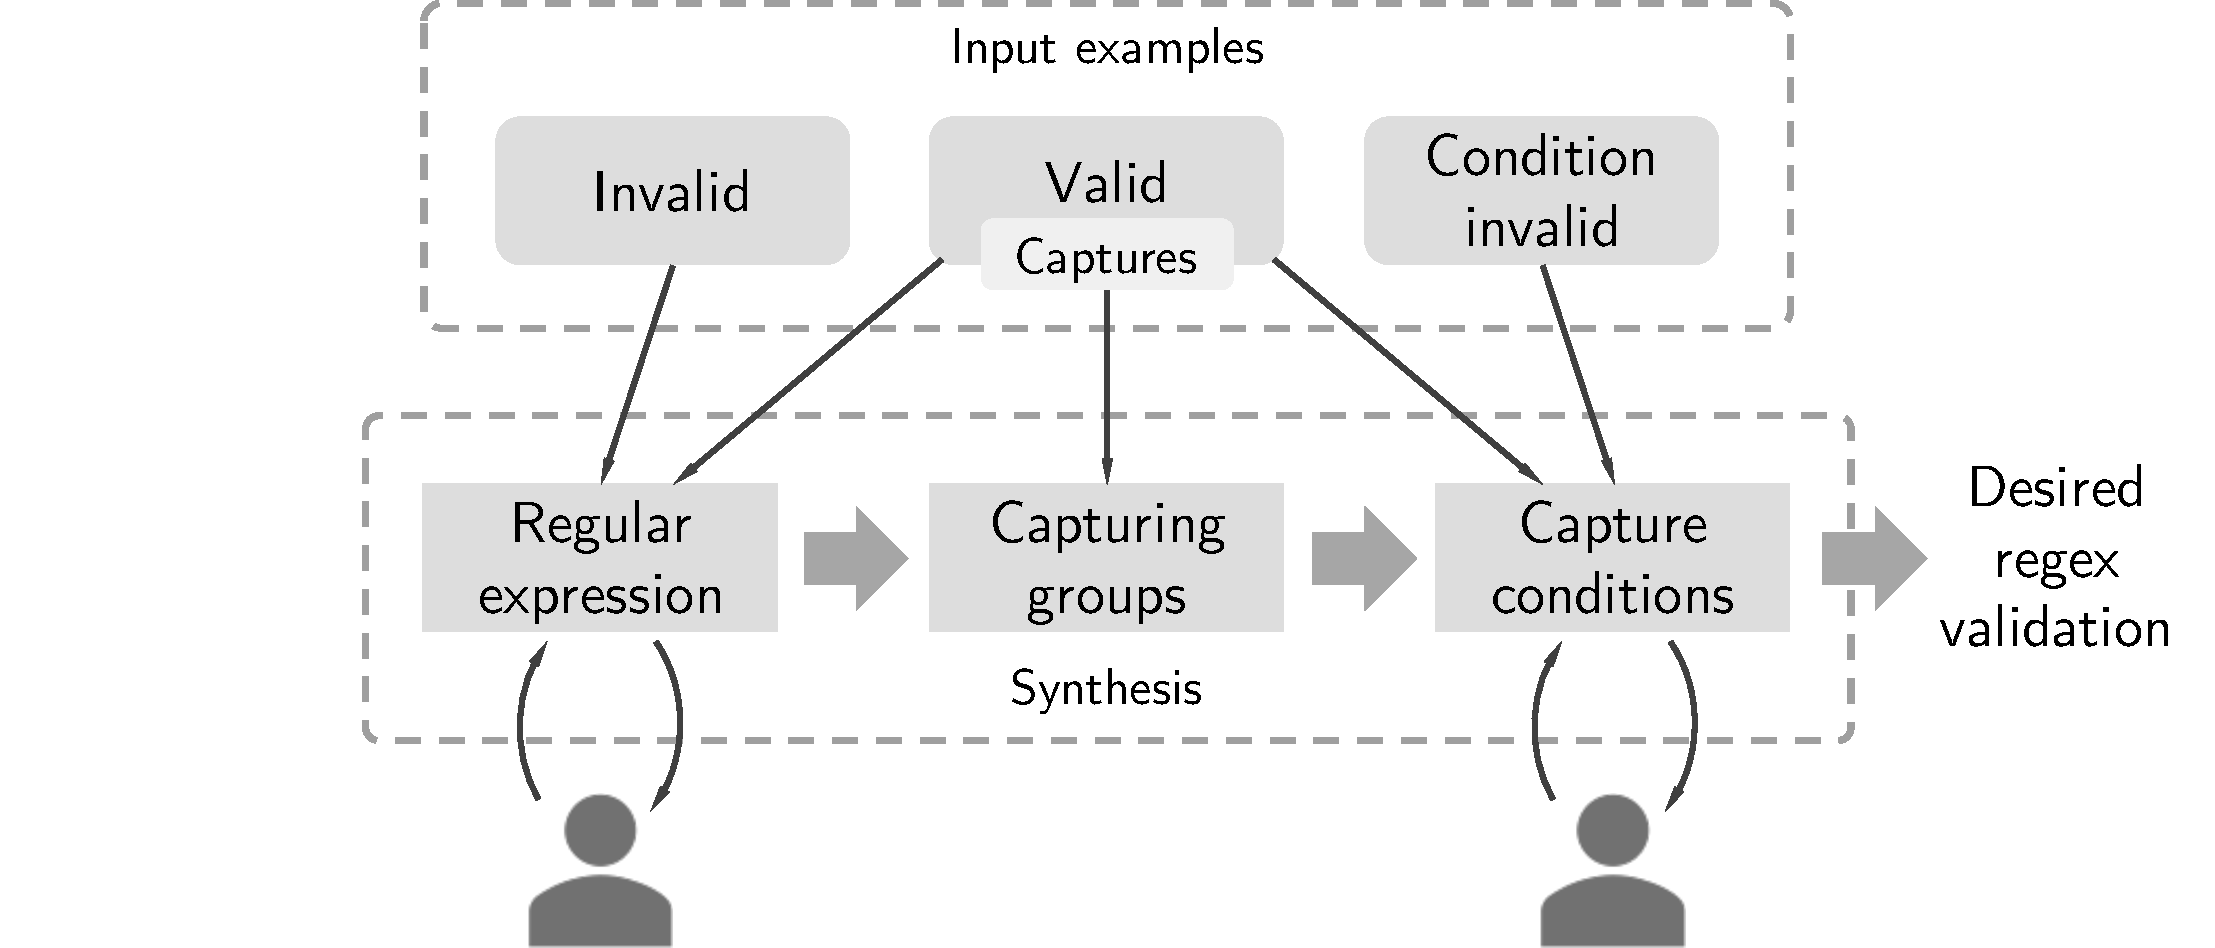
\includegraphics[scale=.35]{pictures/regex_synthesis_h.pdf}
    \caption{\Forest's regex synthesis pipeline}
    \label{fig:regex-synthesis}
\end{figure}

Our synthesis procedure is split into three stages, each relative to an output component. %: regular expression and capture conditions.
First, \Forest synthesises the regular expression, which is the basis for the synthesis of capturing groups.
Secondly, \Forest computes a set of capturing groups that match the captures provided by the used alongside the valid examples. If it is impossible to compute correct capturing groups using the current regular expression, \Forest reverts to the first stage to produce another regular expression.
Finally, \Forest synthesises the capture conditions, by first computing a set of capturing groups and then the conditions to be applied to the resulting captures. Again, if it is not possible to compute correct conditions with the current regular expression, \Forest revers to the first stage to try another regular expression.
\autoref{fig:regex-synthesis} shows the regex validation synthesis pipeline.

All three stages of our synthesis algorithm employ enumerative search, a common approach to solve the problem of program synthesis \cite{DBLP:conf/pldi/FengMBD18,DBLP:conf/pldi/FengMGDC17,AlphaRegex16,Orvalho19,DBLP:conf/cav/ReynoldsBNBT19}.
%
To circumvent the ambiguity of input-output examples,
\Forest{} implements an interaction model.
A new component, the \textit{distinguisher}, ascertains, for any two given programs, whether they are equivalent.
When \Forest finds two different validations that satisfy all examples and are not equivalent, it creates a \textit{distinguishing input}: a new input that has a different output for each solution.
%
To disambiguate between two programs,
\Forest shows the new input to the user, who classifies it as valid or invalid, effectively choosing one program over the other.
%
The new input-output pair is added to the examples, and the enumeration process continues until there is only one solution left.


In summary, we make the following contributions:

\begin{itemize}
    \item We propose a multi-tree SMT representation for regular expressions that leverages the structure of the input example to apply a divide-and-conquer approach.
    
    \item We propose several techniques to prune the search space, based on regex properties.
    
    \item We propose a new method to synthesise capturing groups for a given regular expression and integer conditions over the resulting captures.
    
    \item We implemented our approach in a tool, \Forest{}, that interacts with the user to disambiguate the provided specification. We evaluate \Forest{} on real-world form-validation instances that use regular expressions. Experimental results show that \Forest can synthesise 72\% of the regular expressions that match the user intent.  \Forest{} outperforms \Regel, a general state-of-the-art synthesizer for~regular expressions.
\end{itemize}

\section{Document Structure}

This document is organised as follows.

We begin in~\autoref{chap:background} by introducing some background concepts used throughout the rest of the document. We introduce the concepts of regular language and regular expression, the main logic concepts used throughout this document, and the main components that characterise a program synthesizer.
%
\autoref{chap:program-synthesis} presents a survey of program synthesis algorithms with emphasis on regular expression synthesis.
%
We also look into \textit{AlphaRegex} and \Regel, two regular expression synthesizers that propose optimisations specific to that domain.

We proceed to \autoref{chap:regex-synthesis}, where we take a look into how \Forest synthesises the first part of its regex validation: a regular expression.
%
In \autoref{chap:capture-cond-synthesis} we show how \Forest synthesises the second and third parts of the regex validation: a set of capturing groups that reflect the user-provided captures, and a set of integer conditions over capturing groups that invalidate the conditional invalid examples

We move on to \autoref{chap:results}, where we present and discuss our experiments. We start by comparing \Forest to \Regel, a state-of-the-art regular expression synthesizer. Next, we analyse the time performance of several techniques included in \Forest.
%
Finally, we close up in \autoref{chap:conclusions}, where we summarise the main conclusions of this work, and discuss future directions within this topic.

